\chapter{Experimente}
In diesem Kapitel werden wir drei verschiedenen Beispielen mit sämtliche eingeführten Methoden duchrechnen. Dabei wird zunächst auf die Lösung der Differentialgleichung eingegangen und Konvergenzbetrachtungen durchgeführt. Danach wird der Gradienten des Kostenfunktionals behandelt und die Optimierung für diverse Anfangswerte durchgeführt. %Stay Tuned!
\section{Rolling Stone}
\subsection{Problemstellung}
Zum Anfang wollen wir uns dem sogenannten Rolling Stones Beispiel widmen, welches beispielsweise in \cite{boeck2014experiments} behandelt wurde. 
Es behandelt eine sich reibungslos bewegende Kugel auf einer konvexen Parabel, in dessen Mitte eine flache Ebene auf dem Intervall $[-1,1]$ eingefügt wurde. 
\begin{figure}[ht]
\centering
\begin{minipage}[b]{0.49\linewidth}
% \begin{minipage}[t][3cm][t]{5cm}
\documentclass{standalone}
\IfStandalone{
	\usepackage{pgfplots,pgfplotstable}
	\usetikzlibrary{external}
	
	}{%
}
% \usepackage{pgfplots,pgfplotstable}
% \usetikzlibrary{external}
	

\begin{document}
\tikzsetnextfilename{rolling-stones}
\begin{tikzpicture}[x=3em,y=3em]
\begin{axis}[
            xmin=-2.5,xmax=2.5,
            ymin=-1.5,ymax=1.5,
            xlabel=$z$,
%             legend entries={$V(z)$,$V'(z)$},
            width=\linewidth
        ]
        \addplot[domain=-2.5:-1]{(1+x)^2/2};
        \addplot[-,domain=-1:1]{0};
        \addplot[domain=1:2.5]{(1-x)^2/2};
        \addplot[domain=-2.5:2.5,samples=100,blue]{-min(max(-1-x,0),1-x)};
\end{axis}
\end{tikzpicture}

 
\end{document}

\caption{Rolling Stones}
\label{fig:rollingStones}
\end{minipage}
% \quad
\begin{minipage}[b]{0.49\linewidth}
% \begin{minipage}[t][3cm][t]{5cm}
\documentclass{standalone}
\IfStandalone{
	\usepackage{pgfplots,pgfplotstable}
	\usetikzlibrary{external}
	
	}{%
}
\begin{document}
\tikzsetnextfilename{rolling-stones-solution}
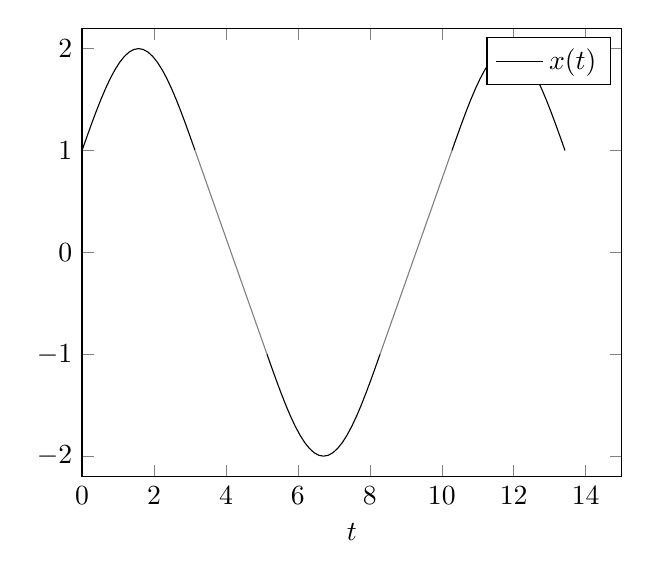
\begin{tikzpicture}[x=3em,y=3em]
\begin{axis}[
            xmin=0,xmax=15,
            ymin=-2.2,ymax=2.2,
            xlabel=$t$,
            legend entries={$x(t)$}
        ]
        \addplot[domain=0:3.14]{1+sin(deg(x))};
        \addplot[domain=pi:pi+2,gray]{1-x+pi};
        \addplot[domain=pi+2:2*pi+2]{-1-sin(deg(2-x))};
        \addplot[domain=2*pi+2:2*pi+4,gray]{x-3-2*pi};
        \addplot[domain=2*pi+4:3*pi+4]{1+sin(deg(x-2*pi-4))};
\end{axis}
\end{tikzpicture} 
\end{document}

\caption{Rolling Stones Lösung}
\label{fig:rollingStonesSolution}
\end{minipage}
\end{figure}
Figur \ref{fig:rollingStones} zeigt die Rampe
\[
 V(z) = \left(\frac{(1+z)^2}{2}\right)\chi_{(-\infty,-1]} + \left(\frac{(1-z)^2}{2}\right)\chi_{[1,\infty)} ,
 ~ \chi_{[a,b)}(z) = 
 \begin{cases}
  1 & z \in [a,b)\\
  0 & \text{sonst}
 \end{cases}
\]

und deren Ableitung, welche wir als gewöhnliche Differentialgleichung mit der Lösung in Figur \ref{fig:rollingStonesSolution} auffassen
 \begin{equation}
  \begin{pmatrix}
   \dot x_1 \\
   \dot x_2 \\
  \end{pmatrix}
 = 
 \begin{pmatrix}
  x_2 \\
  -x_1 - \frac{|x_1-1|}{2} + \frac{|x_1+1|}{2}
 \end{pmatrix}
=F(x)
\label{eq:rolling_stones}
 \end{equation}
wobei $x_1$ die Abszissenposition des Steines und $x_2$ dessen Geschwindigkeit bezeichnet.
Die Funktion \eqref{eq:rolling_stones} ist stückweise linear, sodass wir seine Abs Normal Form \eqref{eq:absNormalForm} angeben können mit
\[
c = \begin{pmatrix}
     -1\\
     1
    \end{pmatrix}
\quad
 Z = \begin{pmatrix}
      1 & 0 \\
      1 & 0
     \end{pmatrix}\quad
J = \begin{pmatrix}
      0&1\\
      -1 & 0
     \end{pmatrix}\quad
 Y = \begin{pmatrix}
      0 & 0\\
      -0.5  & 0.5
     \end{pmatrix}
\]
der Rest wird zu $0$ gesetzt. 


\cite{hasenfelder13}

\subsection{Lösen der ODE}
Die Konvergenz der verallgemeinerten impliziten Mittelpunktsregel 
\begin{figure}
\centering
\documentclass{standalone}
\IfStandalone{
	\usepackage{pgfplots,pgfplotstable}
	\usetikzlibrary{external}
	\newcommand{\fromRoot}[1]{../#1}
}{%
}
\begin{document}
\tikzsetnextfilename{convergence_rolling_plot}
\begin{tikzpicture}
\begin{loglogaxis}[
	width=10cm,
	xlabel=Degrees of freedom $N$,
	ylabel=Error at time $T$,
	legend entries ={Expl. MP,
	IMP,
	GIMP, 
	}
]
  	\addplot[mark=none,red,very thin] table[x index=0,y index=2] {img/data/convergence_rolling_plot.dat};%expl midpoint
 	\addplot[mark=none,green,very thin] table[x index=0,y index=3] {img/data/convergence_rolling_plot.dat};%impl midpoint
	\addplot[mark=none,blue,very thin] table[x index=0,y index=1] {img/data/convergence_rolling_plot.dat};%gen midpoint

	\addplot[mark=none,very thin,gray, yshift=-20pt] 
		table[y={create col/linear regression={x=0,y=1}}] {img/data/convergence_rolling_plot.dat}
		  coordinate [pos=0.5] (A)
		  coordinate [pos=0.6] (B)
		;
	% save the slope parameter:
	\pgfmathparse{-\pgfplotstableregressiona}	
	\pgfmathsetmacro{\slope}{\pgfmathresult}
	
	% draw the opposite and adjacent sides
	% of the triangle
	\draw[very thin,gray] (B) -| (A)
	node [pos=0.2,anchor=north]
	{\pgfmathprintnumber{\slope}};
\end{loglogaxis}
\end{tikzpicture}
\end{document}
\caption{Konvergenz Rolling Stones im Intervall $[0,50]$ mit $x_0=(1,1)$}
\label{fig:rollingStonesConvergence}
\end{figure}

\begin{figure}
\centering
\documentclass{standalone}
\IfStandalone{
	\usepackage{pgfplots,pgfplotstable}
	\usetikzlibrary{external}
	\newcommand{\fromRoot}[1]{../#1}
}{%
}
\begin{document}
\tikzsetnextfilename{convergence_rolling_romberg_plot}
\begin{tikzpicture}
\begin{loglogaxis}[
	width=10cm,
	xlabel=Anzahl der Freiheitsgrade $N$,
	ylabel=Fehler in $x$,
% 	title=Convergence of SWE,
	legend entries ={
% 	Expl. MP,
	IMP,
	GIMP, 
	Romberg Impl,
	Romberg Gen
	}
]
 	\addplot[mark=none,green,very thin] table[x index=0,y index=3] {img/data/convergence_rolling_romberg_plot.dat};%impl midpoint
	\addplot[mark=none,blue,very thin] table[x index=0,y index=1] {img/data/convergence_rolling_romberg_plot.dat};%gen midpoint

	\addplot[mark=none,lime,very thin] table[x index=0,y index=5] {img/data/convergence_rolling_romberg_plot.dat};%Romberg impl midpoint
	\addplot[mark=none,cyan,very thin] table[x index=0,y index=4] {img/data/convergence_rolling_romberg_plot.dat};%ROMBERG gen midpoint
	
	
	\addplot[mark=none,very thin,gray, yshift=-20pt] 
		table[y={create col/linear regression={x=0,y=4}}] {img/data/convergence_rolling_romberg_plot.dat}
		  coordinate [pos=0.5] (A)
		  coordinate [pos=0.6] (B)
		;
	% save the slope parameter:
	\pgfmathparse{-\pgfplotstableregressiona}	
	\pgfmathsetmacro{\slope}{\pgfmathresult}
	
	% draw the opposite and adjacent sides
	% of the triangle
	\draw[very thin,gray] (B) -| (A)
	node [pos=0.2,anchor=north]
	{\pgfmathprintnumber{\slope}};
\end{loglogaxis}
\end{tikzpicture}
\end{document}
\caption{Romberg Konvergenz im Intervall $[0,50]$ mit $x_0=(1,1)$}
\label{fig:rollingStonesConvergenceRomberg}
\end{figure}

Ode Lösung/Romberg
Die in Theorem \ref{thm:convergenceGenMidpoint} vorhergesagte Konvergenzordnung von $\mathcal O(h^2)$. Dass die implizite Mittelpunktsregel eine ebenso hohe Konvergenzrate besitzt liegt daran, dass sie im gegebenen Intervall nur $4$ mal pro $2\pi+4$ Periode Unglattheiten überquert, sonst jedoch normal konvergiert. Aufgrund dieser Unglattheiten entsteht für die implizite Mittelpunktsregel (IMP) kein glatter Konvergenzgraph, sondern sie springt. Demgegenüber konvergiert die verallgemeinerter implizite Mittelpunktsregel (GIMP) sehr stabil, da sie die Knicke der Funktion mit in ihre Berechnung einbezieht.
Insbesondere wird der Fehler der GIMP mit zunehmender Zeit (siehe Fig. \ref{fig:rollingStonesEOT}) nur in den nicht affinen Abschnitten größer während in den affinen Abschnitten exakt gelöst wird, der lokale Fehler der IMP erhöht sich jedoch ständig, bedingt durch die Kinks.
\begin{figure}[ht]
\centering
\documentclass{standalone}
\IfStandalone{
	\usepackage{pgfplots,pgfplotstable}
	\usetikzlibrary{external}
	\newcommand{\fromRoot}[1]{../#1}
}{%
}
\begin{document}
\tikzsetnextfilename{rolling_error_over_time}
\begin{tikzpicture}
\begin{axis}[
	width=\linewidth,
	xlabel=Zeitpunkt $t$,
	ylabel=Fehler zum Zeitpunkt $t$,
	legend entries ={Expl. MP,
	IMP,
	GIMP, 
	},
	legend style={at={(0,1)},anchor=north west}
]
\addplot[mark=none,red,very thin] table[x index=0,y index=3] {img/data/rolling_error_over_time.dat};
\addplot[mark=none,green,very thin] table[x index=0,y index=2] {img/data/rolling_error_over_time.dat};
\addplot[mark=none,blue,very thin] table[x index=0,y index=1] {img/data/rolling_error_over_time.dat};

\end{axis}
\end{tikzpicture}
\end{document}
\caption{Rolling Stones Fehler über Zeit}
\label{fig:rollingStonesEOT}
\end{figure}



\subsection{Adjoints}
Plot adjoints IMP vs GIMP
\subsection{Optimierung}
Convergence
Pfad der Iterationen

\section{LC-Diode}
\cite{boeck2014experiments}
\section{Shallow Water Equation}
\subsection{Problemstellung}
\subsection{Unglattheiten}
Fluxlimiter, Eigenwerte, Plot der Rechten Seite
\subsection{Ergebnisse}


Ein oft genutztes Beispiel, um Datenassimilierungsmethoden zu testen ist die sogenannte Shallow Water Equation (vgl. \cite{zou,navon}). Diese beschreibt die Bewegung einer Flüssigkeit in einem quadratischen Gebiet unter Berücksichtigung von Gravitationswellen. In kartesischen Koordinaten erhält man folgende Gleichungen
\begin{equation}
\begin{aligned}
 \frac{\partial u }{\partial t} = -u\frac{\partial u}{\partial x} -v\frac{\partial u}{\partial y} + fv - \frac{\partial \phi}{\partial x}\\
 \frac{\partial v }{\partial t} = -u\frac{\partial v}{\partial x} -v\frac{\partial v}{\partial y} - fu - \frac{\partial \phi}{\partial y}\\
 \frac{\partial \phi }{\partial t} = -\frac{\partial u\phi}{\partial x} -\frac{\partial v\phi}{\partial y} 
\end{aligned}
\label{eq:swe}
 \end{equation}
Hierbei sind $u$ und $v$ die zwei Komponenten des Fließgeschwindigkeitsfeldes in $s^{-1}$ und $\phi$ das Geopotential in $m^2 s^{-1}$; 
$f$ bezeichnet den Coriolisfaktor.
Die Anfangsbedingungen für die folgenden Experimente wurden aus \cite{grammeltvedt}(6.I) übernommen. Es handelt sich hierbei um eine westwärtgsgerichtete Strömung mit Nord - Süd Störungen verschiedener Wellenlängen und Amplituden entlang der Zonal - Achse der Strömung. Das anfängliche Höhenfeld wurde gewählt mittels Höhenfunktion
\begin{align*}
 h(x,y) = H_0 + H_1 \tanh \left( \frac{9(y-y_0)}{2D}\right) + H_2 \sech^2\left(\frac{9(y-y_0)}{D}\right) \sin\left(\frac{2\pi x}{L}\right)
\end{align*}
und Ableitungen
\begin{align*}
 \frac{\partial h}{\partial x}(x,y) &= h_2\sech^2\left( \frac{9(y-y_0)}{D}\right) \cos\left( \frac{2\pi x}{L} \right)\frac{2\pi}{L} \\
 \frac{\partial h}{\partial y}(x,y) &= h_1 \sech^2\left( \frac{9(y-y_0)}{2D}\right)\frac{9}{2D} -  h_2\frac{18}{D} \sin\left( \frac{2\pi x}{L}\right) \frac{\sinh(9(y-y_0)/D)}{\cosh^3(9(y-y_0)/D)}\\
\end{align*}
wobei $D$ die Breite, $L$ die Länge der betrachteten Fläche ist,  $h_0 := 2000m$, $h_1 := -220m$, $h_2 := 133m$ und $y_0 = D/2$. Als schlussendliche Anfangsbedingungen ergeben sich
\begin{align*}
 \phi_0(x,y) &= gh(x,y)\\
 u_0(x,y) &= -\frac{f}{g} \frac{\partial h}{\partial y}(x,y)\\
 v_0(x,y) &= \frac{f}{g} \frac{\partial h}{\partial x}(x,y)
\end{align*}
mit $f := 10^{-4} s^{-1}$ und $g:= 10 ms^{-1}$.
Damit wir die Datenassimilierungsmethode auf (\ref{eq:swe}) anwenden können, müssen wir die Gleichung in eine Form überführen, welche nur noch von der Zeit $t$ abhängt. Grammeltvedt (in \cite{grammeltvedt}) bietet dazu diverse Finite Differenzen Schematas für die Shallow Water Equation an, mit denen sich \ref{eq:swe} in die gewünschte Form überführen lässt. In unserem Fall nutzen wir Schema F. (\ref{eq:swe}) erhält somit die Form:
\begin{equation}
 \begin{aligned}
  \frac{\partial u}{\partial t} &= -(\bar{u}^x\bar{u}^x)_x - (\bar{u}^y\bar{v}^y)_y + u(\bar{u}^x_x+ \bar{v}^y_y) +fv - \bar{\phi}^x_x\\
  \frac{\partial v}{\partial t} &= -(\bar{v}^x\bar{u}^x)_x - (\bar{v}^y\bar{v}^y)_y + v(\bar{u}^x_x+ \bar{v}^y_y) -fv - \bar{\phi}^y_y\\
  \frac{\partial \phi}{\partial t} &= -(\bar{\phi}^x\bar{u}^x)_x - (\bar{\phi}^y\bar{v}^y)_y   
 \end{aligned}
 \label{eq:schemef}
\end{equation}
mit \[
\begin{aligned}
\overline{(uv)}^x_x & = \bar{u}^{2x} \bar{v}^x_x +\bar{v}^{2x} \bar{u}^x_x \\
(\bar{u}^z\bar{v}^z)_z &= \frac{1}{2} \left[ \overline{(uv)}^x_x + u \bar{v}^x_x + v \bar{u}^x_x \right] \\
 &= \frac{1}{2} \left[ \bar{u}^{2x}\bar{v}^x_x +  \bar{v}^{2x}\bar{u}^x_x  + u \bar{v}^x_x + v \bar{u}^x_x \right]\\
 \bar{u}^x_x &= \frac{1}{\Delta} \left[ \bar{u}^x(x_i+\frac{\Delta}{2}) -\bar{u}^x(x_i-\frac{\Delta}{2})  ) \right]\\
	    &=  \frac{1}{2\Delta} \left[ u(x_i+\Delta)+u(x_i)-u(x_i)-u(x_i-\Delta) \right]\\
	    &=  \frac{1}{2\Delta} \left[ u(x_i+\Delta)-u(x_i-\Delta) \right]\\
 \bar{u}^{2x}&= \frac{1}{2} \left[ u(x_i+\Delta) + u(x_i - \Delta)\right]
\end{aligned}
\]
Mit diesen Gleichungen können wir das Schema programmieren. Die Randbedingungen sind durch starre homogene Neumannbedingungen entlang der Nord- und Süd Grenzen und periodischen Randbedingungen bezüglich der Ost/West Grenzen gegeben. Seien $x_l,x_r,y_t,y_b$ die Koordinaten bzgl. der linken (l), rechten (r), oberen (t) und unteren (b) Ränder. Dann sind die Randbedingungen folgendermaßen definiert:
\begin{equation}
 \begin{aligned}
  u(x_l,y,t) = u(x_r,y,t)\\
  v(x_l,y,t) = v(x_r,y,t)\\
  \phi(x_l,y,t) = \phi(x_r,y,t)\\
  \frac{\partial u}{\partial y}(x,y_t,t) = 0 = \frac{\partial u}{\partial y}(x,y_b,t)\\ 
  v(x,y_t,t) = 0 = v(x,y_b,t)\\
  \frac{\partial \phi}{\partial y}(x,y_t,t) = 0 = \frac{\partial \phi}{\partial y}(x,y_b,t)\\ 
 \end{aligned}
\end{equation}
